% A results and discussion section which integrates answers to the questions above, assignment of spectra, 
% includes a discussion of yields and data collected. It is useful if you include subheadings etc to draw attention to 
% the answers you provide to the questions.

% As large volumes of data are generated or extensive calculations will be done, the results of these need 
% to be presented in an appropriate style (graph, table or figure) and these results need to be described 
% and discussed in the context of the experimental aims.


\subsection{Electron Transfer Kinetics via Emission Spectroscopy}
\subsubsection*{Results}
SEE APPENDIX MEI REF LATER
structure discussion in paragraphs

\begin{figure}[H]
    \centering
    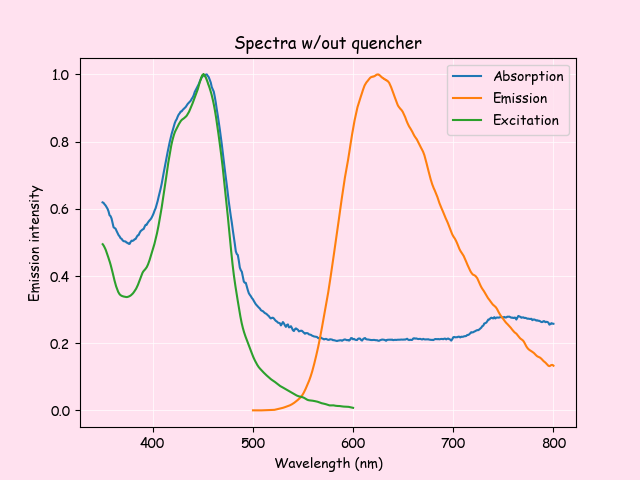
\includegraphics[width = 0.7\linewidth]{part1_noq.png}
    \caption{Absorption, emission, and excitation spectra of \ce{Rubpy^{2+}}}
    \label{fig:part1_noq}
\end{figure}
\begin{figure}[H]
     \centering
     \begin{subfigure}[b]{0.49\textwidth}
         \centering
         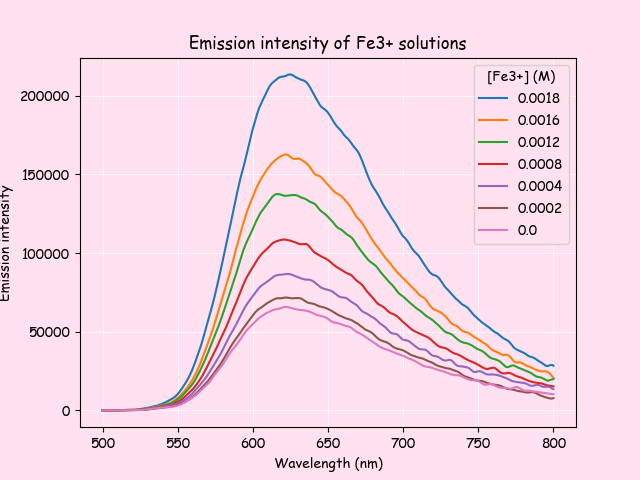
\includegraphics[width=\textwidth]{part1_fe.png}
         \caption{\ce{Fe^{3+}}}
         \label{fig:part1_fe}
     \end{subfigure}
     \hfill
     \begin{subfigure}[b]{0.49\textwidth}
         \centering
         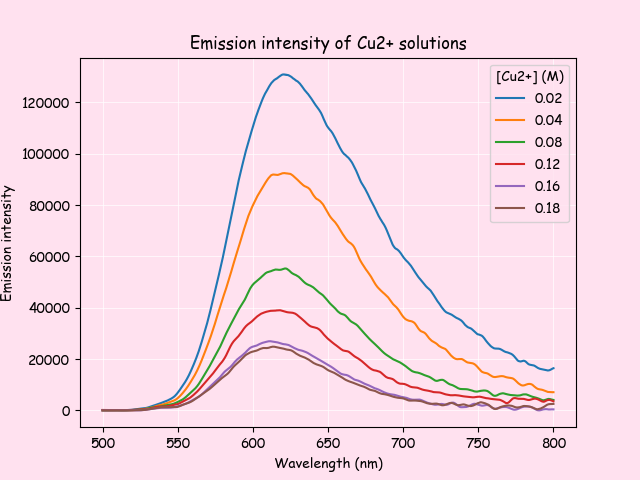
\includegraphics[width=\textwidth]{part1_cu.png}
         \caption{\ce{Cu^{2+}}}
         \label{fig:part1_Cu}
     \end{subfigure}
     \caption{Emission spectra in the presence of quencher molecules}
     \label{fig:part1_fecu_spectra}
\end{figure}
Figure \ref{fig:part1_fecu_spectra} shows that for both \ce{Fe^{3+}} and \ce{Cu^{2+}}, as concentration increases, the wavelength at which peak emission intensity occurs does not change, but intensity increases with concentration.
\\
\textbf{Question 1}
\begin{figure}[H]
     \centering
     \begin{subfigure}[b]{0.49\textwidth}
         \centering
         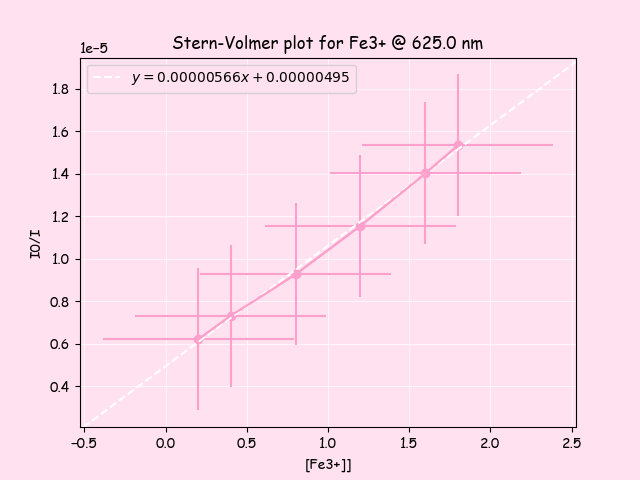
\includegraphics[width=\textwidth]{part1_q1_Fe.png}
         \caption{\ce{Fe^{3+}}}
         \label{fig:part1_q1_fe}
     \end{subfigure}
     \hfill
     \begin{subfigure}[b]{0.49\textwidth}
         \centering
         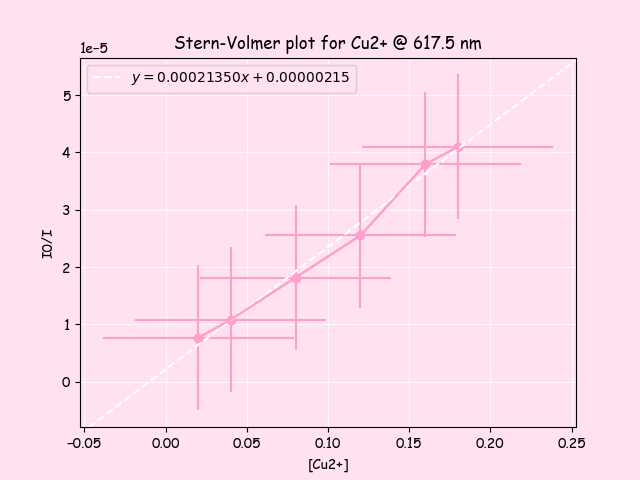
\includegraphics[width=\textwidth]{part1_q1_Cu.png}
         \caption{\ce{Cu^{2+}}}
         \label{fig:part1_q1_Cu}
     \end{subfigure}
     \caption{Stern-Volmer plots for luminescent quenching measurements}
     \label{fig:stern_volmers}
\end{figure}
\par Figure \ref{fig:stern_volmers} represents the following curve (eqn (6) from lab manual\autocite{lab_manual}):
\begin{equation*}
    \frac{I_0}{I} = 1 + \frac{k_q}{k_d}[Q]
\end{equation*}

So $\frac{k_q}{k_d}$ is the slope of each curve, which are:
\begin{equation*}
    \mathcolorbox{Lavender}{\frac{dy}{dx}_{\text{Fe}^{3+}} = \input{part1_q1_fe_slope.txt} \text{ @ } \input{part1_q1_fe_wl.txt} \text{ nm} }
\end{equation*}
\begin{equation*}
    \mathcolorbox{Lavender}{\frac{dy}{dx}_{\text{Cu}^{2+}} = \input{part1_q1_cu_slope.txt} \text{ @ } \input{part1_q1_cu_wl.txt} \text{ nm} }
\end{equation*}
\\
\textbf{Question 2}
\par From the lab manual\autocite{lab_manual}, $k_d = 1.7 \times 10^6\text {s}^{-1}$. Thus,
\begin{equation}
    k_q = \text{slope} \times k_d
    \label{eq:p1q2}
\end{equation}
Substituting slopes to equation (\ref{eq:p1q2}):
\begin{equation*}
    \mathcolorbox{Lavender}{k_{q,\text{Fe}^{3+}} = \input{part1_q2_fe.txt} \text{ s}^{-1}}
\end{equation*}
\begin{equation*}
    \mathcolorbox{Lavender}{k_{q,\text{Cu}^{2+}} = \input{part1_q2_cu.txt} \text{ s}^{-1}}
\end{equation*}
\\
\textbf{Question 3}
\par From tables 2 and 3 in the lab manual\autocite{lab_manual}:
   $ k_{11} = 1 \times 10 ^ 8 \text{ M}^{-1}\text{s}^{-1}$, 
    $k_{22, \text{Fe}^{3+}} = 4 \text{ M}^{-1}\text{s}^{-1}$, 
    $k_{22, \text{Cu}^{2+}} = 1 \times 10 ^ {-5} \text{ M}^{-1}\text{s}^{-1}$. And standard reduction potentials: $E^{\circ}_{\text{R}^{3+}} = -0.8 \text{ V}$, $E^{\circ}_{\text{Fe}^{3+}} = 0.77 \text{ V}$, $E^{\circ}_{\text{Cu}^{2+}} = 0.16 \text{ V}$.
\\ Since $E^{\circ}_{\text{Cell}} = E^{\circ}_{\text{Red}} + E^{\circ}_{\text{Ox}}$, 
\begin{equation}
    E^{\circ}_{\text{Cell}} = E^{\circ}_{\text{Red}} + 0.8 \text{ V}
    \label{eq:ecell}
\end{equation}
Rearranging equations (13) and (12) respectively from the lab manual\autocite{lab_manual},
\begin{equation}
    K_{12} = e^{\frac{zF}{RT}E^{\circ}_{\text{Cell}}} \text{ } 
    \label{eq:K12}
\end{equation}
\begin{equation}
    f_{12} = e^{\frac{(\ln{K_{12}})^2}{4\ln{(k_{11}k_{22} / Z_{12}^2)}}}
    \label{eq:f12}
\end{equation}
Equation (11) from the lab manual\autocite{lab_manual} gives:
\begin{equation}
    k_{\text{ET}} = k_{12} \approx \sqrt{k_{11}k_{22}K_{12}f_{12}}
    \label{eq:ket}
\end{equation}
Where $Z_{12} \approx 10^{11} \text{ M}^{-1} \text{s}^{-1}$, $T = 298.15\text{ K}$, $R = 8.3145\text{ Jmol}^{-1}\text{K}^{-1}$and $F = 96485.3399 \text{ Cmol}^{-1}$.
\\
\par The \textcolor{Lavender}{\mintinline{Python}{kET(k22, x_red_potential, z)}} Python function (see Appendix \ref{appx:part1_code} for full script) takes inputs for ($k_{22}$, $E^{\circ}_{\text{Red}}$, $z$), and substitutes above given values, equations (\ref{eq:ecell}), (\ref{eq:K12}), and (\ref{eq:f12}) to equation (\ref{eq:ket}), to return the $k_{\text{ET}}$ value.
% \input{marcus_theory_fn.txt}
This function was called for ($k_{22 \text{Fe}^{3+}}$, $E^{\circ}_{\text{Fe}^{3+}}$, $z = 1$), and ($k_{22, \text{Cu}^{2+}}$, $E^{\circ}_{\text{Cu}^{2+}}$, $z = 1$) to respectively return
\begin{equation*}
    \mathcolorbox{Lavender}{k_{\text{ET},\text{Fe}^{3+}} = \input{part1_q3_fe.txt} \text{ M}^{-1} \text{s}^{-1}}
\end{equation*}
\begin{equation*}
    \mathcolorbox{Lavender}{k_{\text{ET},\text{Cu}^{2+}} = \input{part1_q3_cu.txt} \text{ M}^{-1} \text{s}^{-1}}
\end{equation*}

\subsubsection*{Discussion Questions}
\begin{enumerate}
%
    \item 
\end{enumerate}

% 1. Describe and explain the similarities and/or differences between the absorption, emission, and
% excitation spectra of Ru(bpy)32+∗. (Hint: Use Figure 2.)

% 2. Normalise the emission spectra to the maximum emission intensity for each Fe3+ and Cu2+ concen-
% tration in the luminescence quenching measurements. What happens to the shape of the spectra as the Fe3+ or Cu2+ concentration increases? Why? (Hint: Plot the absorption spectra of one of the Fe3+-containing samples and one of the Cu2+-containing samples and compare them to the
% absorption spectrum of the pure Rubpy2+ sample).

% 3. Compare the quenching rate coefficients obtained from the Stern–Volmer plots with the electron-
% transfer rate coefficients calculated from Marcus theory and comment on any similarities or differ-
% ences. Note that the rate coefficient for diffusion-controlled collisions between electron-transfer
% partners under the conditions studied is ∼3.3 × 109 M−1 s−1.

% 4. Compare the rate coefficients for Fe3+ and Cu2+ (both experimental and calculated) and explain the
% similarities or differences.

\subsection{Part 2}
\subsubsection*{Results}
SEE APPENDIX MEI REF LATER
\subsubsection*{In Class Analysis}
\textbf{Question 1}
\begin{figure}[H]
     \centering
     \begin{subfigure}[b]{0.49\textwidth}
         \centering
         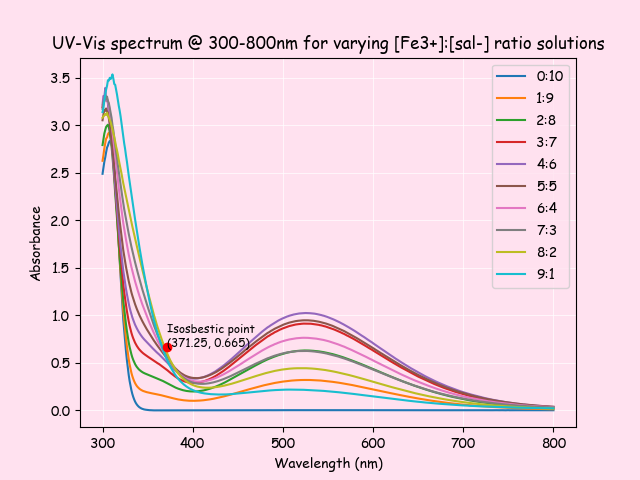
\includegraphics[width=\textwidth]{part2_q1a.png}
         \caption{RENAME}
         \label{fig:part2_q1_a}
     \end{subfigure}
     \hfill
     \begin{subfigure}[b]{0.49\textwidth}
         \centering
         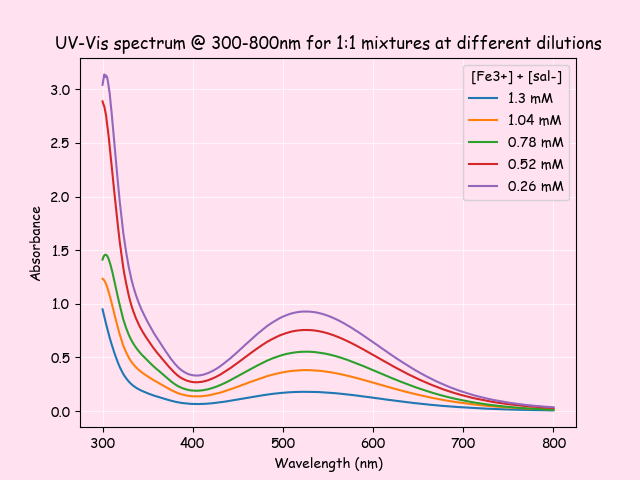
\includegraphics[width=\textwidth]{part2_q1_b.png}
         \caption{REDO}
         \label{fig:part2_q1_b}
     \end{subfigure}
     \caption{sjdfsdn}
     \label{fig:part2q1}
\end{figure}
Isosbestic point was found to be \hl{$\input{part2_q1a.txt}\unskip$}, by averaging the points of intersection for each subsequent solution for those where Fe$^{3+}$ is in excess (6:4 - 10:1). (See Appendix \ref{appx:part2_code} for Python code)
\\
\textbf{Question 2}
\begin{figure}[H]
    \centering
    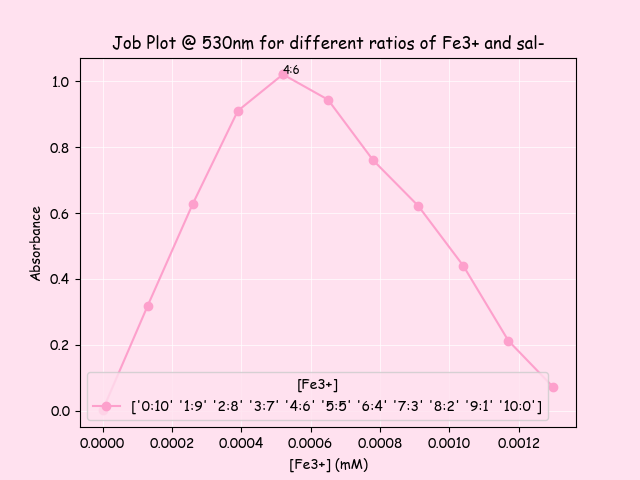
\includegraphics[width = 0.6\linewidth]{part2_q2_job_plot.png}
    \caption{Caption}
    \label{fig:part2q2}
\end{figure}
The ratio at which the peak of Job plot occured was at a ratio of \input{part2_q2.txt}\unskip. Thus, the mpirical formula of the complex was found to be:
\begin{equation}
\mathcolorbox{Lavender}{\ce{(Fe^{3+})_{4}(sal^-)_6}}
    \label{eq:emp_formula}
\end{equation}
\\
\textbf{Question 3}
\begin{figure}[H]
    \centering
    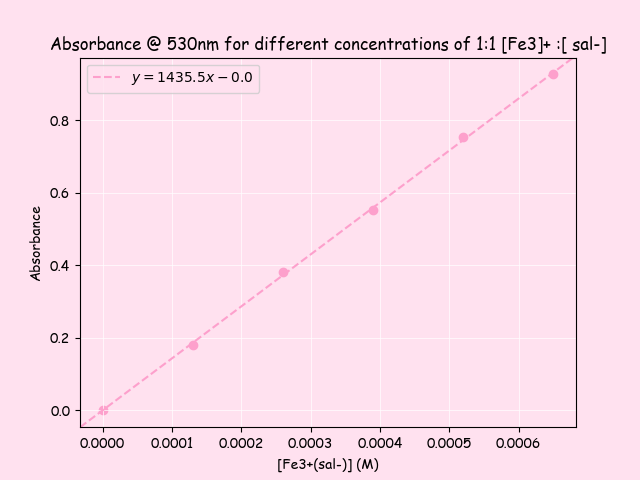
\includegraphics[width = 0.6\linewidth]{part2_q3.png}
    \caption{Caption}
    \label{fig:part2q3}
\end{figure}
\subsubsection*{Discussion Questions}
\begin{enumerate}
    \item Analysis was conducted at the absorbance maximum of the \ce{FUCK} complex as larger absorbance values allow for more reliable comparison of data. Additionally, as shown in Figure \ref{fig:part2_q1_a}, the absorbance maximum for varying ratios remains the same, despite the shape of the curve changing with ratio. Thus, the wavelength at which peak absorption occurs is the most appropriate as this peak is common across all solution ratios.
    \item this is fucking jail
    \item wavelength at which isosbestic point occurs is roughly extinction coefficient multiplied by absorbance max (explain but also keep length of cuvette oin mind)
\end{enumerate}
% 1. Why is the absorption maximum of the complex at 530 nm an appropriate wavelength at which to
% do the analysis to determine the empirical formula and stability constant of the complex?

% 2. Compare the values of the molar extinction coefficient and stability constant of the complex
% calculated using the two different calculation methods. Discuss any similarities or differences.
% Comment on the relative accuracy of the two methods.

% 3. Determine the relationship between the molar extinction coefficient of Fe3+ and Fe3+(sal – ) at
% the isosbestic point in the measurements of different mixture ratios. (Hint: Because the stability
% constant K is very large, you can assume that the complex formation reaction essentially goes to
% completion. You should also use the fact that the total added concentration of Fe3+ and sal – is the
% same in all samples.






